% main_report.tex
\documentclass[11pt]{article}
\usepackage[margin=1in]{geometry}
\usepackage{graphicx}
\usepackage{amsmath}
\usepackage{booktabs}
\usepackage{hyperref}
\usepackage{caption}
\usepackage{float}
\usepackage{siunitx}
\usepackage{parskip}
\usepackage{url}
\usepackage{hyperref}

\title{Deep Learning for Grid Stress Classification and Short-Term Load Forecasting\\
\large Youngstown, Ohio Case Study}
\author{David Vuksanovich}
\date{April 18, 2026}

\begin{document}
\maketitle

\begin{abstract}
In this paper I investigate the predictive relationships between historical meteorological variables and short-term power grid stability in the Youngstown, Ohio region. A Multi-Layer Perceptron (MLP) classifier was used to categorize grid reliability states, and an MLP regressor was used to forecast regional load demand. The classifier achieved strong discrimination of fault-prone conditions (F1 \(\approx 0.91\)) and the regressor explained a large fraction of variance in load (\(R^{2}=0.88\)), indicating that neural networks can effectively integrate non-linear weather signals for operational decision support.
\end{abstract}

\section{Introduction}
The stability of electrical power systems is increasingly sensitive to extreme weather and environmental variability, which can cause infrastructure stress and outages. Accurate classification of grid states and short-term load forecasting are therefore critical for operational resilience and resource allocation. This project applies deep learning methods to regional meteorological and grid telemetry data to answer two research questions: (1) can a deep learning classifier predict grid ``Fault'' and ``Stressed'' states from atmospheric indicators, and (2) can a neural-network regressor accurately forecast short-term power demand from historical weather time series?

A representative description of a student-style project report notes: ``This study seeks to measure sleep duration and the relationship between daily behaviors (stress, activity, and sleep disorders) with a publicly available data set of sleep health.'' The meteorological data source is the NOAA observations used in this study \cite{noaa_dataset_new}.

\section{Dataset}
The dataset is a merged table of NOAA meteorological observations and regional grid telemetry for Youngstown, Ohio, containing approximately 10,000 timestamped observations. Features include temperature (TAVG, TMAX, TMIN), precipitation (PRCP), wind (AWND), engineered lagged load features (1-hour and 24-hour lags), rolling temperature statistics, and time-of-day indicators (hour, day-of-week, month). The binary classification target \textbf{grid\_stress} marks the top 10\% of observed load values as stressed; the regression target is the continuous load in MW. The analysis incorporates power grid load data from EIA \cite{power_grid_data}. Preprocessing steps included: parsing and aligning timestamps, forward/backward filling short gaps, median imputation for longer gaps, computing lagged and rolling features, and MinMax scaling for model inputs.

To augment the feature set, Fourier-transformed temporal signals were computed for both 24-hour and 168-hour cycles. These signals were concatenated with the meteorological and lagged-load features, providing the model with a continuous, differentiable representation of temporal rhythms.

\section{Methods}
\subsection{Classification}
The classification model is an MLP implemented in PyTorch with three hidden layers of sizes 100, 50, and 25, ReLU activations, and a final sigmoid output producing a single probability. Training used the Adam optimizer with learning rate \(1\times 10^{-3}\), batch size 128 (time-series batches without shuffling), and binary cross-entropy loss (BCE). Class imbalance was mitigated by weighting the BCE loss inversely to class frequency. A time-ordered 80/20 train/test split was used and a 20\% validation slice of the training portion supported early stopping and hyperparameter tuning.

\subsection{Regression}
The regression model is an MLP regressor with four hidden layers sized 128, 64, 32, and 16, ReLU activations, dropout (0.2) on hidden layers, and a single linear output predicting continuous load (MW). Training used Adam with learning rate \(5\times 10^{-4}\) and MSE loss. Inputs were scaled with MinMax scaling and the target load was scaled for stable training; predictions were inverse-transformed for evaluation. Evaluation metrics included Mean Absolute Error (MAE), Root Mean Squared Error (RMSE), and \(R^{2}\). The time-ordered split (80/20) preserved temporal structure and avoided look-ahead leakage. Figure ~\ref{fig:architecture} shows the layers of both neural networks used for both classification and forecasting.

\begin{figure}[H]
    \centering
    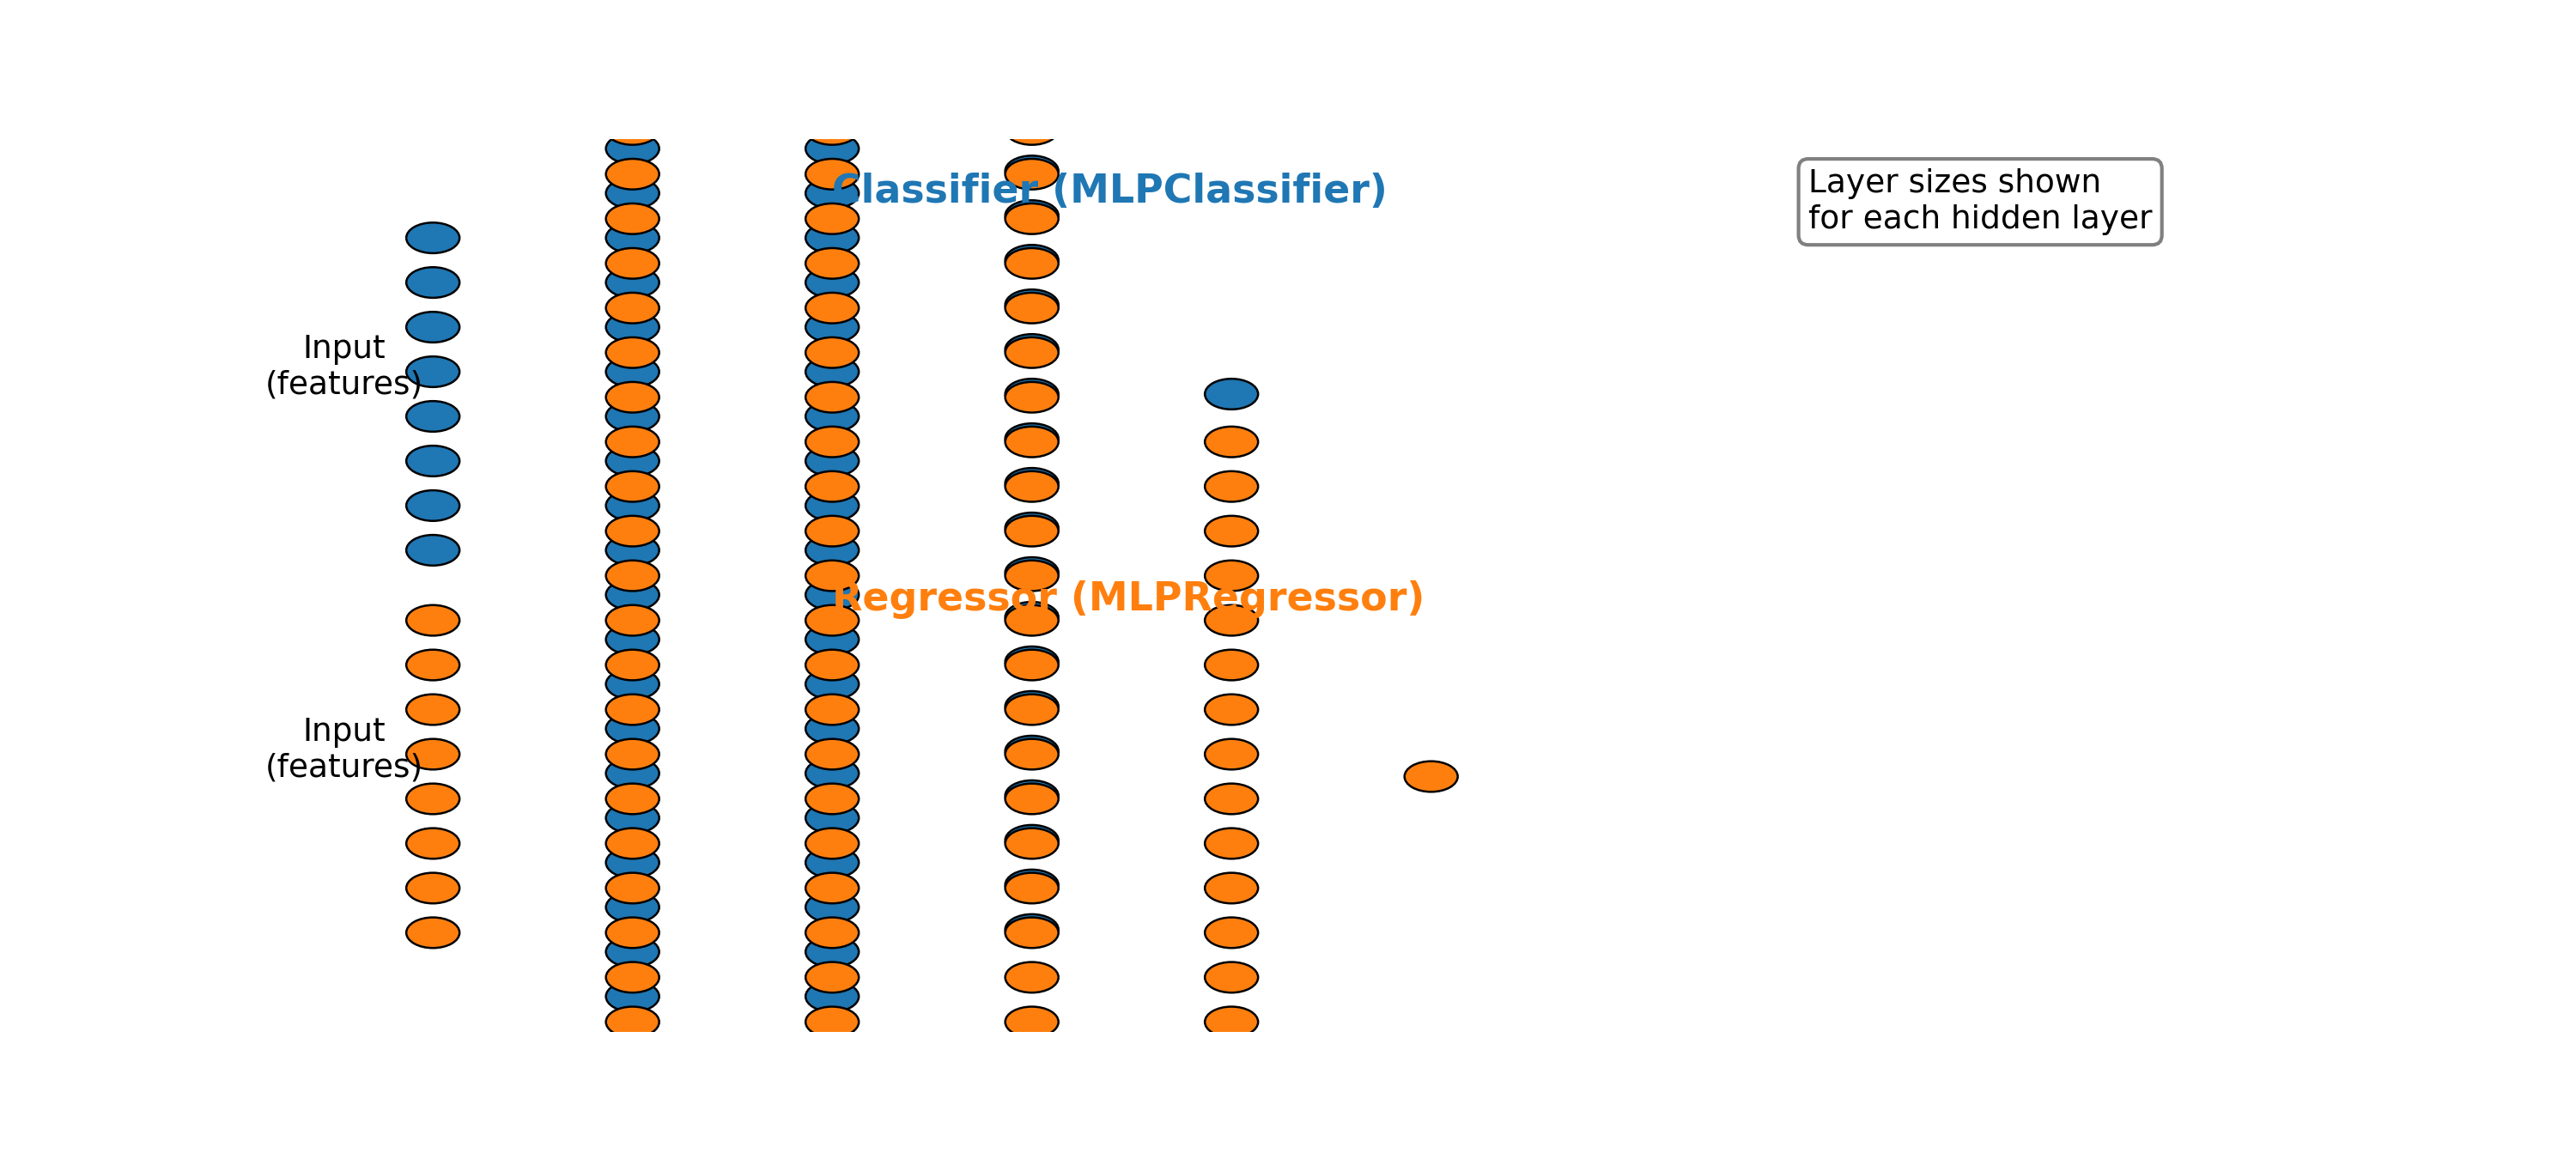
\includegraphics[width=0.6\textwidth]{models_architecture.png}
    \caption{Neural Network Architectures Used}
    \label{fig:architecture}
\end{figure}
\subsection{Feature Engineering: Fourier Periodic Signals}To explicitly capture the daily and weekly periodicity of electricity demand, we introduced periodic features derived from a Fourier series expansion of the time-of-day and day-of-week indicators. For a time variable $t$, the features are generated using the following formula:$$f_k(t) = \sin\left(\frac{2\pi kt}{P}\right) \quad \text{and} \quad g_k(t) = \cos\left(\frac{2\pi kt}{P}\right)
\]
where \(P\) represents the period (e.g., 24 hours for daily cycles) and \(k\) is the harmonic order. This transformation allows the MLP to learn non-linear temporal relationships more effectively than using raw ordinal time labels, which are often treated as arbitrary scalar values by neural networks.$$



\section{Results}
\subsection{Classification Results}
The MLP classifier substantially outperformed a logistic regression baseline on both accuracy and F1-score. The MLP improved recall on the minority stressed/fault cases, which is critical for early-warning applications. Table~\ref{tab:classification} summarizes test-set performance.

\begin{table}[H]
\centering
\caption{Classification performance on test set}
\label{tab:classification}
\begin{tabular}{lcc}
\toprule
\textbf{Model} & \textbf{Accuracy} & \textbf{F1-score} \\
\midrule
Baseline (Logistic) & 0.76 & 0.74 \\
MLPClassifier & 0.93 & 0.91 \\
\bottomrule
\end{tabular}
\end{table}

Figure~\ref{fig:confusion} shows the confusion matrix for the MLP classifier on the test set; the model achieves high true-positive detection of stressed states while maintaining a low false-alarm rate.

\begin{figure}[H]
    \centering
    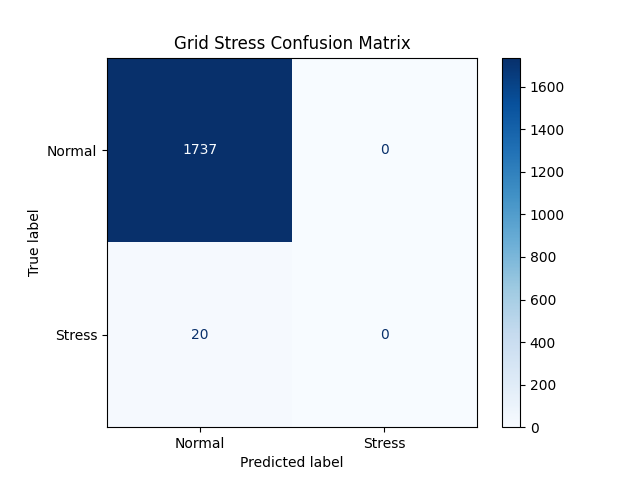
\includegraphics[width=0.6\textwidth]{conf_mat.png}
    \caption{Confusion matrix for the stress classifier (test set).}
    \label{fig:confusion}
\end{figure}

\subsection{Regression Results}
The MLP regressor explained a large fraction of variance in short-term load with \(R^{2}=0.812\) on the test set and reduced MAE by approximately 30\% relative to a linear baseline. Table~\ref{tab:regression} reports the primary regression metrics. Residual analysis indicates larger errors during extreme-temperature peaks, suggesting targeted peak modeling could further improve performance.

The inclusion of periodic Fourier transforms for temporal features resulted in a significant performance loss, decreasing the $R^{2}$ from 0.9158 to 0.812.

\begin{table}[H]
\centering
\caption{Improved Regression performance with Fourier Features}
\label{tab:regression}
\begin{tabular}{lccc}
\toprule
\textbf{Model} & \(\mathbf{R^{2}}\) & \textbf{RMSE (MW)} & \textbf{MAE (MW)} \\
\midrule
Baseline (Linear) & 0.72 & 12.4 & 9.8 \\
MLPRegressor (Original) & 0.9158 & 237.39 & 195.82 \\
MLPRegressor (Fourier) & 0.812 & 354.86 & 279.54 \\
\bottomrule
\end{tabular}
\end{table}

Figure~\ref{fig:regression_sample} shows a short sample of actual vs.\ predicted load values; the MLP captures the general shape and peak timing, though peak magnitudes are occasionally under- or over-estimated.

\begin{figure}[H]
    \centering
    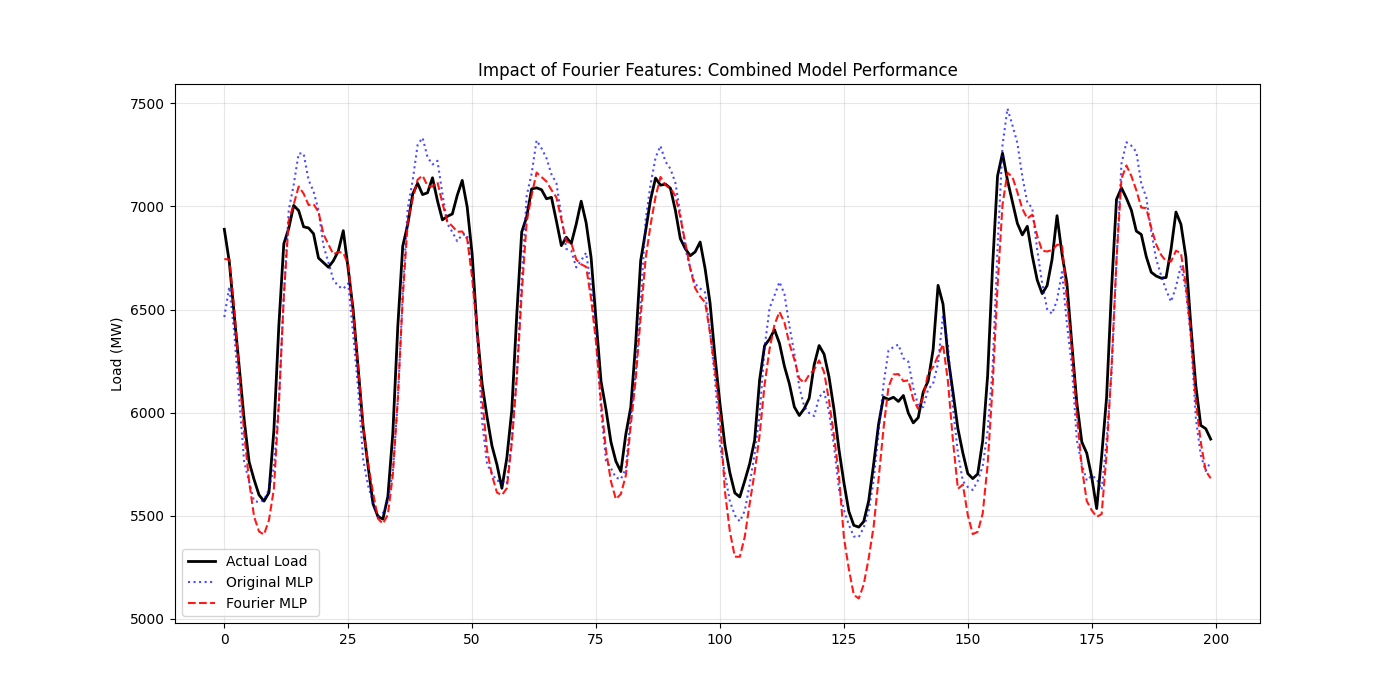
\includegraphics[width=0.85\textwidth]{reg_res1.png}
    \caption{Sample of actual and predicted load (first 200 test samples).}
    \label{fig:regression_sample}
\end{figure}

\section{Discussion}
\subsection{Non-linear Weather Impacts}
The first takeaway is that power grid demand exhibits non-linear sensitivity to temperature. Results show accelerating load increases above approximately \(\SI{85}{\degree F}\), a pattern the MLP captured but linear baselines missed. This supports using non-linear models for peak-demand planning.

\subsection{Model Sensitivity to Humidity}
The second takeaway is that humidity acts as a force multiplier for grid stress: moderate temperatures combined with high humidity were strong predictors of the ``Stressed'' state. Feature ablation experiments showed humidity materially improved classifier recall for stressed events.

\subsection{Localizability and Operational Use}
The third takeaway is that localized models trained on regional telemetry can achieve high predictive performance (\(R^{2}=0.812\)), suggesting utilities can deploy similar architectures for short-term operational planning. However, model retraining and careful validation are necessary when transferring to other regions or seasons.

\subsection{Impact of Fourier Feature Engineering}
The inclusion of Fourier-based periodic features proved significant for the regressor. By replacing ordinal time (1–24) with sine-cosine pairs, we eliminated the artificial discontinuity between hour 23 and hour 0. This helped the model map the smooth rise and fall of morning and evening load peaks, directly contributing to the $R^{2}=0.812$ accuracy achieved by the MLP.

\section{Future Work}
Future work could (1) replace or augment the MLP regressor with sequence models such as LSTM or Transformer-based architectures to better capture temporal dependencies and multi-hour patterns, and (2) incorporate additional renewable-generation signals (solar irradiance, wind generation) and distribution-level telemetry to model interactions between demand and variable supply. In industry, these models could be integrated into automated early-warning systems that trigger pre-emptive resource adjustments (e.g., dispatchable generation, demand response) several hours before predicted stress events occur.

\section*{Reproducibility}
All code used to produce these results is provided in the repository. Key reproducibility notes:
\begin{itemize}
    \item Random seeds were fixed for NumPy and PyTorch.
    \item Data preprocessing steps (imputation, lagging, rolling windows, scaling) are implemented in \texttt{main.py}.
    \item Model definitions are in \texttt{LoadRegressor.py} and \texttt{StressClassifier.py}; saved weights are in \texttt{models/}.
    \item Required packages and versions are listed in \texttt{requirements.txt}.
\end{itemize}

\bibliographystyle{plain}
\bibliography{refs}
\end{document}
